
%=============================================================================
\section{Higher Level Components}
\label{sec:ddg4-implementation-higher-level-components}
%=============================================================================
\noindent
Layered components, which base on the general framework implement higher 
level functionality such as the handling of Monte-Carlo truth associations
between simulated energy deposits and the corresponding particles or the
generic handling of input to the simulation.

\noindent
To generalize such common behavior it is mandatory that the participating
components collaborate and understand the data components they commonly access.
The data model is shown in Figure~\ref{fig:ddg4-event-data-model}.
\begin{figure}[t]
  \begin{center}
    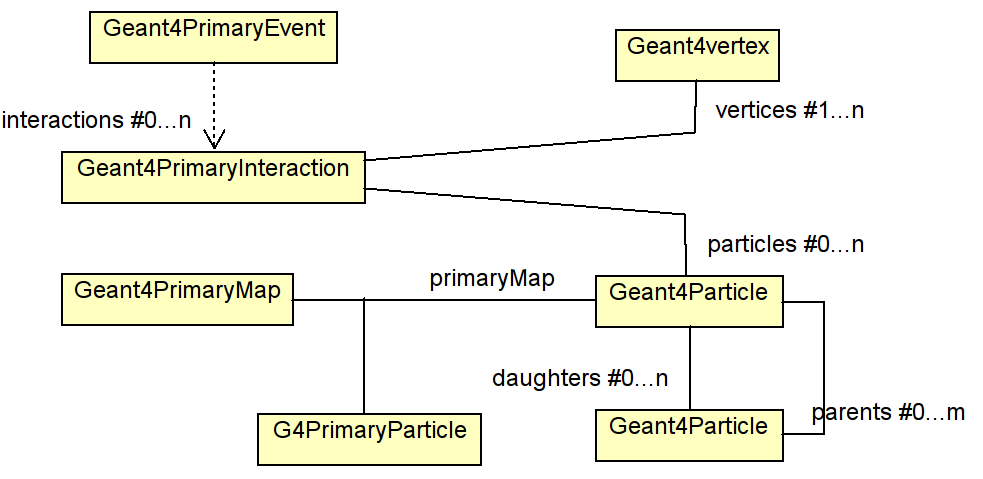
\includegraphics[width=120mm] {DDG4_event_data_model}
    \caption{The DDG4 event data model.}
    \label{fig:ddg4-event-data-model}
  \end{center}
\end{figure}

\noindent
{\bf{Please note}}, that this data model  is by no means to be made persistent 
and used for physics user analysis. This model is optimized to support
the simulation process and the necessary user actions to handle MC truth,
to easily and relatively fast look up and modify parent-daughter 
relationships etc. This choice is based on the assumption, that the 
additional overhead to convert particles at the input/output 
stage is small compared to the actual resource consumption of Geant4
to simulate the proper detector response.
On the other hand this choice has numerous advantages:
\begin{itemize}\itemcompact
\item Accepting the fact to convert input records allows to adapt 
  DDG4 in a simple and flexible manner to any input format. Currently 
  supported is the input from raw {\tts{LCIO}} files, {\tts{StdHep}} 
  records using {\tts{LCIO}} and {\tts{ASCII}} files using the 
  {\tts{HEPEvt}} format.
\item Similarly as for the input stage, also the output format 
  can be freely chosen by the clients.
\item No assumptions was made concerning the structure to store 
  information from energy deposits. Any information extract produced
  by the sensitive actions can be adapted provided at the output
  stage the proper conversion mechanism is present. The sensitive 
  detectors provided by DDG4 are {\bf{optional only and by no means mandatory}}.
  User defined classes may be provided at any time. Appropriate tools
  to extract MC truth information is provided at the output stage.
\item The modular approach of the action sequences described 
  in~\ref{sec:ddg4-user-manual-implementation-geant4action-sequences}
  allows to easily extend the generation sequence to handle multiple 
  simultaneous interactions, event overlay or spillover response 
  very easily~\footnote{The handling of spillover is only possible 
  if during the digitization step the correct signal shape corresponding
  to the shift of signal creation is taken into account.}
\end{itemize}

\noindent
In section~\ref{sec:ddg4-implementation-input-handling} the generic mechanism
of input data handling is described. \\
In section~\ref{sec:ddg4-implementation-particle-handling} the MC truth 
handling is discussed. \\
In section~\ref{sec:ddg4-implementation-output-handling} we describe the 
output mechanism.
\newpage

%=============================================================================
\subsection{Input Data Handling}
\label{sec:ddg4-implementation-input-handling}
%=============================================================================
\begin{figure}[t]
  \begin{center}
    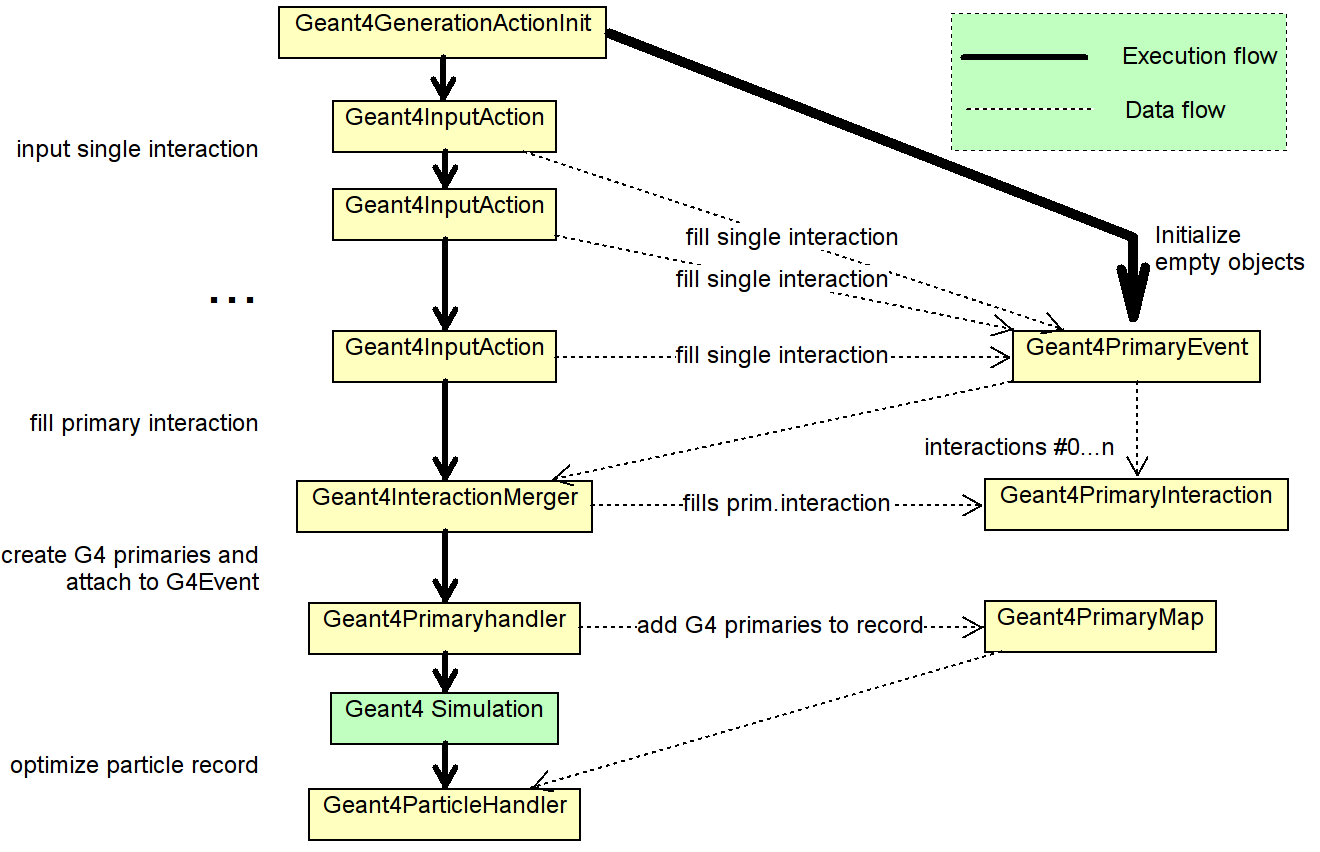
\includegraphics[width=160mm] {DDG4_input_stage}
    \caption{The generic handling of input sources to DDG4.}
    \label{fig:ddg4-input-stage}
  \end{center}
\end{figure}

\noindent
Input handling has several stages and uses several modules:
\begin{itemize}\itemcompact
\item First the data structures \tts{Geant4PrimaryEvent}, 
    \tts{Geant4PrimaryInteraction} and \tts{Geant4\-Primary}\-\tts{Map} are initialized 
    by the action \tts{Geant4GenerationActionInit} 
    and attached to the {\tts{Geant4Event}} structure.
\item The initialization is then followed by any number of input modules.
  Typically each input module add one interaction. Each interaction has a 
  unique identifier, which is propagated later to all particles. Hence all
  primary particles can later be unambiguously be correlated to one of the 
  initial interactions. 
  Each instance of a \tts{Geant4InputAction} creates and fills a separate instance
  of a \tts{Geant4PrimaryInteraction}.
  In section~\ref{sec:ddg4-implementation-geant4inputaction} the functionality and
  extensions are discussed in more detail.
\item All individual primary interactions are then merged to only single record
  using the \tts{Geant4}\-\tts{Interaction}\-\tts{Merger} component.
  This components fills the \tts{Geant4PrimaryInteraction} registered to the
  \tts{Geant4Event}, which serves as input record for the next component,
\item the \tts{Geant4PrimaryHandler}. The primary handler creates the proper 
  \tts{G4PrimaryParticle} and \tts{G4PrimaryVertex} objects passed to \tts{Geant4}.
  After this step all event related user interaction with Geant4 has completed,
  and the detector simulation may commence.
\end{itemize}
All modules used are subclasses of the {\tts{Geant4}\-\tts{Generator}\-\tts{Action}} and must be
added to the \tts{Geant4}\-\tts{Generator}\-\tts{Action}\-\tts{Sequence} as described 
in~\ref{sec:ddg4-user-manual-implementation-geant4action-sequences}.

\noindent
An object of type {\tts{Geant4PrimaryEvent}} exists exactly once for 
every event to be simulated. The empty {\tts{Geant4PrimaryEvent}} is created by the
{\tts{Geant4GenerationActionInit}} component. All higher level components may then 
access the {\tts{Geant4PrimaryEvent}} object and subsequently an individual interaction
from the {\tts{Geant4Context}} using the extension mechanism as shown in 
the following code:
\begin{code}
/// Event generation action callback
void SomeGenerationComponent::operator()(G4Event* event)  {
  /// Access the primary event object from the context
  Geant4PrimaryEvent* evt = context()->event().extension<Geant4PrimaryEvent>();
  /// Access the container of interactions
  const std::vector<Geant4PrimaryEvent::Interaction*>& inter = evt->interactions();
  /// Access one single interaction to be manipulated by this component
  Geant4PrimaryInteraction* evt->get(m_myInteraction_identifier);
  ....
\end{code}
{\bf{Please note:}} To keep components simple, each component should 
only act on one interaction the component has to uniquely identify.
The identification may be implemented by e.g. an access mask passed to the 
component as a property.

%=============================================================================
\subsection{Anatomy of the Input Action}
\label{sec:ddg4-implementation-geant4inputaction}
%=============================================================================
\noindent
One input action fills one primary interaction.
\tts{Geant4InputAction} instances may be followed by decorators, which 
allow to to smear primary vertex (\tts{Geant4InteractionVertexSmear}) or
to boost the primary vertex \tts{Geant4InteractionVertexBoost} and all 
related particles/vertices.


Please note, that a possible reduction of particles in
the output record may break this unambiguous relationship between 
"hits" and particles.
......

%=============================================================================
\subsection{Monte-Carlo Truth Handling}
\label{sec:ddg4-implementation-particle-handling}
%=============================================================================
As any other component in \DDG, the   was
designed using the plugin mechanism ie. the default implementation
which was inspired by the original implementation of the MC thruth
handler developed by the Linear Collider community may easily be
overloaded.

\noindent
The Monte-Carlo thruth handler takes care that 
\begin{itemize}
\item the proper MC particles are associated with the corresponding hits
      and tracks.
\item To compress the particle record. Geant4 creates a large amount 
      of temporary particles in particluar in dense areas of the 
      detector such as calorimeters. In calorimeters however, the 
      hits within a confined volume should be assigned to the incoming
      track. In addition a track is only supposed to be kept if it 
      satisfies certain criteria.
\end{itemize}
To achieve this functionality the Monte-Carlo thruth handler implemented
in the class \tts{Geant4ParticleHandler} firstly
\begin{itemize}
\item implements the interface \tts{Geant4MonteCarloTruth} which gets
      called whenever an interaction occurs in a sensitive volume
      which is modeled by an instance of a instance of 
      \tts{Geant4SensitiveAction}.
\item to properly manager the MC particle records the 			
	  \tts{Geant4ParticleHandler} either inherits or uses
	  the callbacks provided by the DDG4 interfaces to the
	  \begin{itemize}
		  \item \tts{Geant4GeneratorAction}
		  \item \tts{Geant4EventAction}
		  \item \tts{Geant4TrackingAction}
		  \item \tts{Geant4SteppingAction}.
	  \end{itemize}
	  While the response of one track is simulated, all relevant 
	  information is extracted in the callbacks and at the end of the
	  simulation of the track response a decision is taken whether to
	  store the information of the Geant4 track in the MC particle
	  record or not.
\item A Geant4 track is saved in the MC track record if
	  \begin{itemize}
	  	  \item the track did not intercat with the detector, but 
	  	  		is part of the Monte-Carlo record originating
	  	  		from the original generator consisting of quarks,
	  	  		leptons, gluons, gammas etc.
		  \item the track was declared to Geant4 as a Geant4 primary
		        track from the generator action. These are either 
		        long-living remnants of the underlying hard interaction
		        of particles decaying macroscopically inside the
		        experiment volume like e.g. B-mesons.
		  \item the track exits the world volume.
		  \item the track is mother particle to secondaries.
		  \item the track created a hit in a \it{"tracker"}-type
		        sensitive volume.
		  \item the track is above a certain energy threshold and
		  		has at least one associated hit either in a 
		  		\it{calorimter}-type volume of a \it{tracker}-type
		  		volume.
	  \end{itemize}
	  For all tracks purged from the MC particle record, any resulting
	  energy deposit is associated to the last parent particle 
	  stored in the MC particle record.
\item To fine-tune the Monte-Carlo truth handler in \DDG a 
	  use class with interface  \tts{Geant4UserParticleHandler} 
	  may be supplied, which allows to customize and fine tune
	  if a given MC particle is supposed to be kept in the final
	  record or not. This user class receives the identical callbacks
	  as the truth handler, but at the end of the simulation of each
	  track (the end-tracking-action) a call is issued by the truth
	  handler and allows to override the decision whether to keep
	  or dismiss storing a track.
\end{itemize}

\noindent
As mentioned above this implementation is only an example how
to realize such a Monte-Carlo truth logic. It is assumed that the
interface \tts{Geant4ParticleHandler} together with the easy-to-use
subscription mechanism to all callbacks provided by Geant4
allow to easily implement other Monte-Carlo truth mechanisms.

\vspace{0.3cm}
\noindent
The following table shows all properties accepted by the 
\DDG Monte-Carlo truth handler.

\vspace{0.3cm}
\noindent
\begin{tabular}{ l p{10cm} }
\hline
\bold{Class name}      & \tts{Geant4ParticleHandler}           \\
\bold{File name}       & \tts{DDG4/src/Geant4ParticleHandler.cpp} \\
\bold{Type}            & \tts{Geant4Action}                                  \\
\hline 
\bold{Component Properties:}   & defaults apply                              \\
\bold{PrintEndTracking} (bool) & \tts{Extra printout at the end of the } \\
                               & \tts{tracking action for debugging} \\
\bold{PrintStartTracking} (bool) & \tts{Extra printout at the start of the } \\
                               & \tts{tracking action for debugging} \\
\bold{KeepAllParticles} (bool) & \tts{Flag to override any NC particle removal} \\
\bold{SaveProcesses} (bool)    & \tts{Save all produces of the specified} \\
                               & \tts{Geant4 particle processes} \\
\bold{MinimalKineticEnergy} (bool)  & \tts{Minimal energy cut required to accept a MC particle} \\
\bold{MinDistToParentVertex} (bool) & \tts{Minimal distance to the parent's }\\
                               & \tts{start-vertex in order to become an independent particle} \\
                               & \tts{Used to e.g. suppress Delta-rays} \\
\end{tabular}

\newpage

%=============================================================================
\section{Output Data Handling}
\label{sec:ddg4-implementation-output-handling}
%=============================================================================

\noindent
The output of the data record of the accepted MC particle record
and the corresponding sets of hits in the various subdetectors is 
basic to further handing data originating from simulated particle
collisions. In \DDG the handling of output data is implemented as
a specialization of a \tts{Geant4EventAction} since the output
needs to written at the end of each simulated event.

\noindent
Currently there are three types of output formats implemented:
\begin{itemize}
\item Writing the MC particle record and the Geant4 hits
	  natively as ROOT objects to a ROOT file.
	  This is a very simple solution, writes the entire event
	  as a ROOT TTree object. The persistent data format of the 
	  objects is the same as the transition data format in memory
	  used during the simulation step.
\item Writing the particle record and the hit structures in LCIO 
      data format. For details of the LCIO data format
      please consult the LCIO manual.
\item Writing the particle record and the hit structures in 
      the EDMS data format developed by the CERN/SFT data format.
      For details of the LCIO data format please consult the LCIO
      manual.
\end{itemize}

Unless the native ROOT format is used for data output,
the data format of the transient representation 
of Monte-Carlo particles and the resulting tracker- and
calorimeter hits differes from the persistent representation 
and requires data conversion. The overheads of such conversions however
are typically neglidgeble with respect to the rather large resource
usage required for simulation.

\vspace{0.3cm}
\noindent
The component properties of the generic output class:

\vspace{0.3cm}
\noindent
\begin{tabular}{ l p{10cm} }
\hline
\bold{Class name}      & \tts{Geant4OutputAction}           \\
\bold{File name}       & \tts{DDG4/src/Geant4OutputAction.cpp} \\
\bold{Type}            & \tts{Geant4Action}                                  \\
\hline 
\bold{Component Properties:}   & defaults apply                              \\
\bold{Output} (string) & \tts{String representation of the output-file} \\
\bold{HandleErrorsAsFatal} (bool) & \tts{Convert any error of the concrete implementation}\\
                                  & \tts{into a fatal exception causing \DDG to stop processing.}\\
\end{tabular}

\vspace{0.3cm}
\noindent
The component properties of the ROOT output class:

\vspace{0.3cm}
\noindent
\begin{tabular}{ l p{10cm} }
\hline
\bold{Class name}      & \tts{Geant4Output2ROOT}           \\
\bold{File name}       & \tts{DDG4/src/Geant4Output2ROOT.cpp} \\
\bold{Type}            & \tts{Geant4Action}                                  \\
\hline 
\bold{Component Properties:}   & defaults apply                              \\
\bold{Section} (string)        & \tts{Name of the ROOT TTree to store the event data.}\\
                               & \tts{Default: EVENT} \\
\bold{HandleMCTruth} (bool)    & \tts{Handle the results of the Monte-Carlo thruth handler}\\
                               & \tts{when outputting data}\\
\bold{DisabledCollections}     & \tts{vector<string>}\\
                               & \tts{Geant4 filled collections, which should be excluded}\\
                               & \tts{from the output record.}\\
\bold{DisableParticles} (bool) & \tts{Inhibit the output of the particle record.}
                               
\end{tabular}


\newpage
